\documentclass[a4paper,11pt]{article}

\usepackage[T1]{fontenc}
\usepackage[utf8]{inputenc}
\usepackage{graphicx}
\usepackage{xcolor}

\renewcommand\familydefault{\sfdefault}
\usepackage{tgheros}

\usepackage{amsmath,amssymb,amsthm,textcomp}
\usepackage{enumerate}
\usepackage{multicol}
\usepackage{tikz}
\usepackage{pdfpages}


\graphicspath{ {.} }
\usepackage{geometry}
\geometry{left=25mm,right=25mm,%
bindingoffset=0mm, top=20mm,bottom=20mm}



\usepackage{tabularx,lipsum,environ,amsmath,amssymb}

\makeatletter
\newcommand{\problemtitle}[1]{\gdef\@problemtitle{#1}}% Store problem title
\newcommand{\problemquestion}[1]{\gdef\@problemquestion{#1}}% Store problem question
\newcommand{\problemsolution}[1]{\gdef\@problemsolution{#1}}% Store problem input
\NewEnviron{problem}{
  \problemtitle{}\problemquestion{}\problemsolution{}% Default input is empty
  \BODY% Parse input
  \par\addvspace{.5\baselineskip}
  \noindent
  \begin{tabularx}{\textwidth}{@{\hspace{\parindent}} l X c}
    \multicolumn{2}{@{\hspace{\parindent}}l}{\@problemtitle} \\% Title
    \textbf{Description:} & \@problemquestion \\% Question
        \textbf{Solution:} & \@problemsolution % Input
  \end{tabularx}
  \par\addvspace{.5\baselineskip}
}
\makeatother







\linespread{1.3}

\newcommand{\linia}{\rule{\linewidth}{0.5pt}}

% custom theorems if needed
\newtheoremstyle{mytheor}
    {1ex}{1ex}{\normalfont}{0pt}{\scshape}{.}{1ex}
    {{\thmname{#1 }}{\thmnumber{#2}}{\thmnote{ (#3)}}}

\theoremstyle{mytheor}
\newtheorem{defi}{Definition}

% my own titles
\makeatletter
\renewcommand{\maketitle}{
\begin{center}
\vspace{2ex}
{\huge \textsc{\@title}}
\vspace{1ex}
\\
\linia\\
\@author \hspace{100ex} m.plevako@innopolis.university \hspace{100ex} BS18-02 \hspace{100ex} Variant (c)

\vspace{4ex}
\end{center}
}
\makeatother
%%%

% custom footers and headers
\usepackage{fancyhdr}
\pagestyle{fancy}
\lhead{}
\chead{}
\rhead{}
\lfoot{Assignment \textnumero{} 3}
\cfoot{}
\rfoot{Page \thepage}
\renewcommand{\headrulewidth}{0pt}
\renewcommand{\footrulewidth}{0pt}
% 

% code listing settings
\usepackage{listings}
\lstset{
    language=Python,
    basicstyle=\ttfamily\small,
    aboveskip={1.0\baselineskip},
    belowskip={1.0\baselineskip},
    columns=fixed,
    extendedchars=true,
    breaklines=true,
    tabsize=4,
    prebreak=\raisebox{0ex}[0ex][0ex]{\ensuremath{\hookleftarrow}},
    frame=lines,
    showtabs=false,
    showspaces=false,
    showstringspaces=false,
    keywordstyle=\color[rgb]{0.627,0.126,0.941},
    commentstyle=\color[rgb]{0.133,0.545,0.133},
    stringstyle=\color[rgb]{01,0,0},
    numbers=left,
    numberstyle=\small,
    stepnumber=1,
    numbersep=10pt,
    captionpos=t,
    escapeinside={\%*}{*)}
}

%%%----------%%%----------%%%----------%%%----------%%%

\begin{document}

\title{HW \textnumero{} 3}

\author{Matvey Plevako}

\maketitle


\section*{Problem 1}

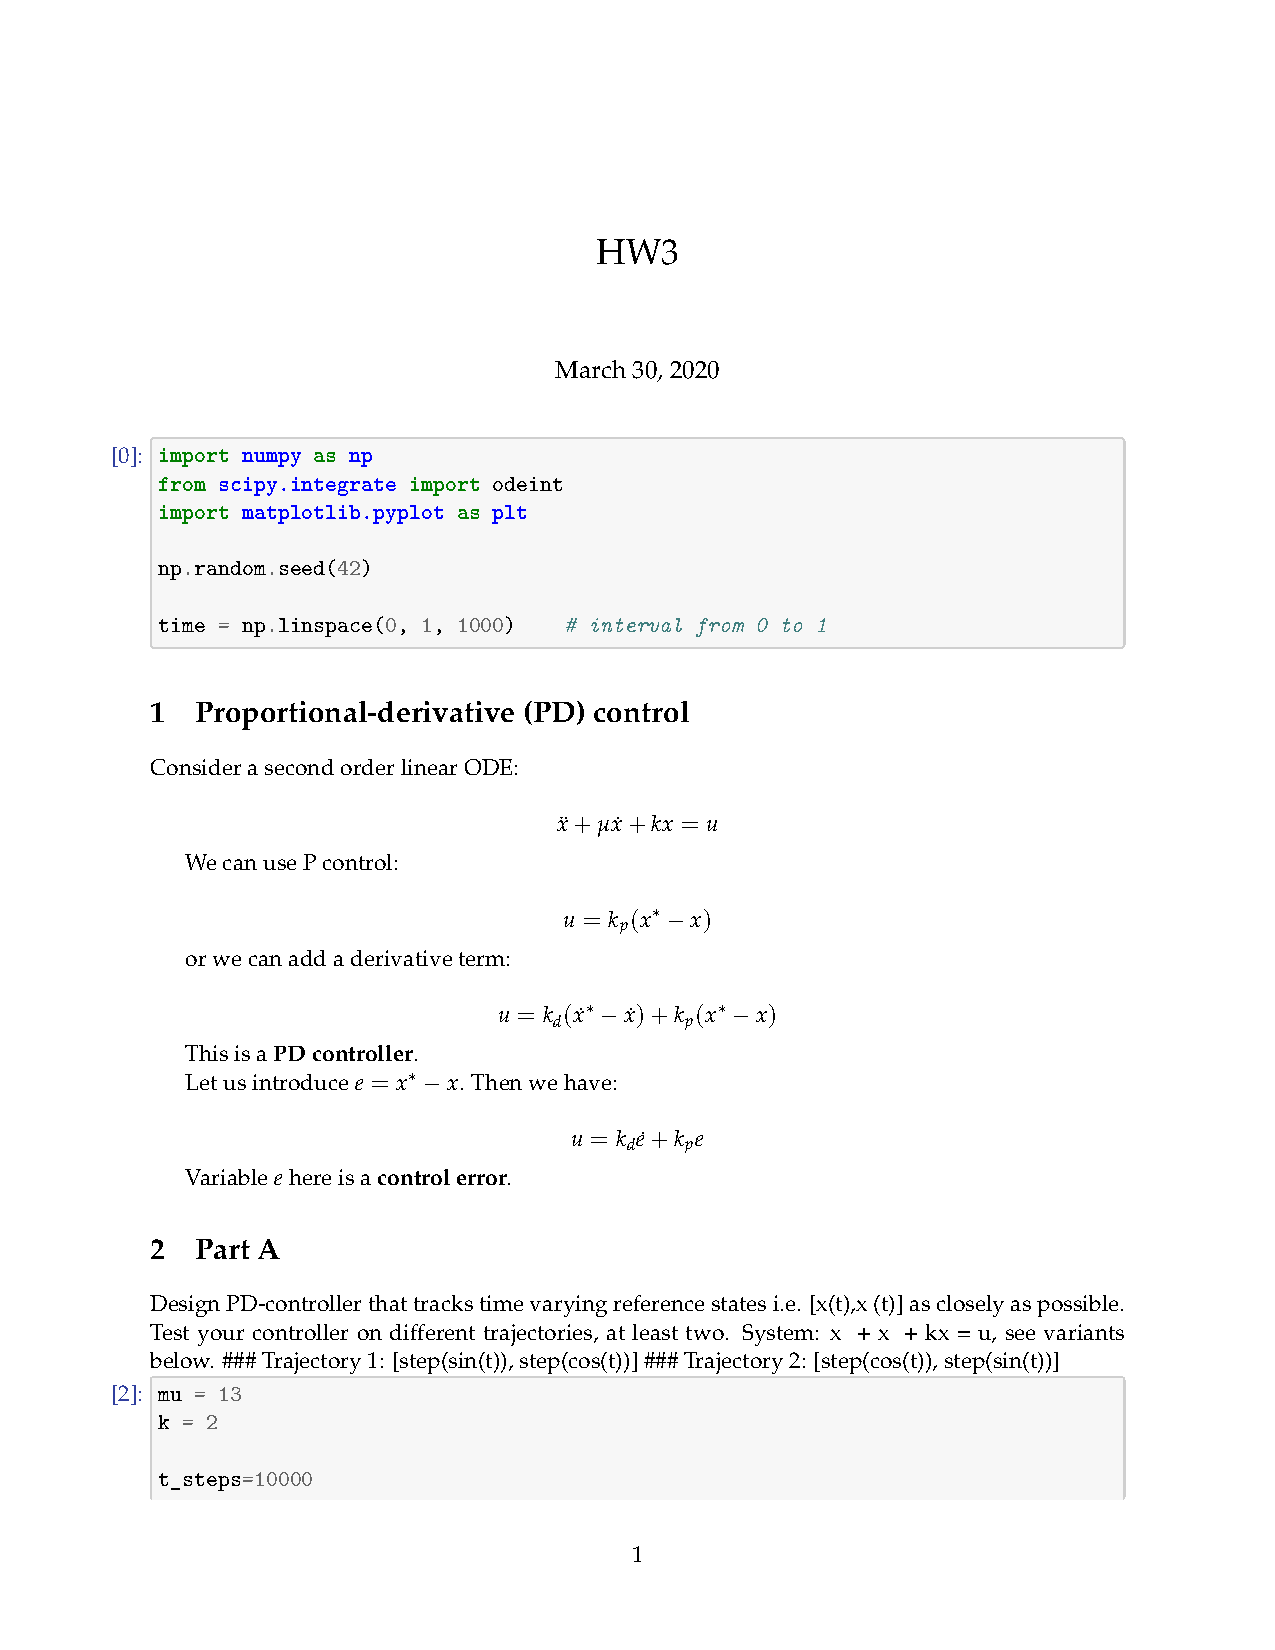
\includepdf[pages=-]{HW3_task1.pdf}


\section*{Problem 2}
$$W(s) = \frac{s+1}{s^3+2s^2 + 9s + 20}$$
\begin{problem}
  \problemquestion{Design a PID controller. Use step input function and try to improve rise time, overshoot and steady-state error, comparing with no controller system. Describe your actions. Use pidTuner in Matlab.}
\end{problem}
1. Design Simulink scheme with Transfer Function and PID controller
$$$$
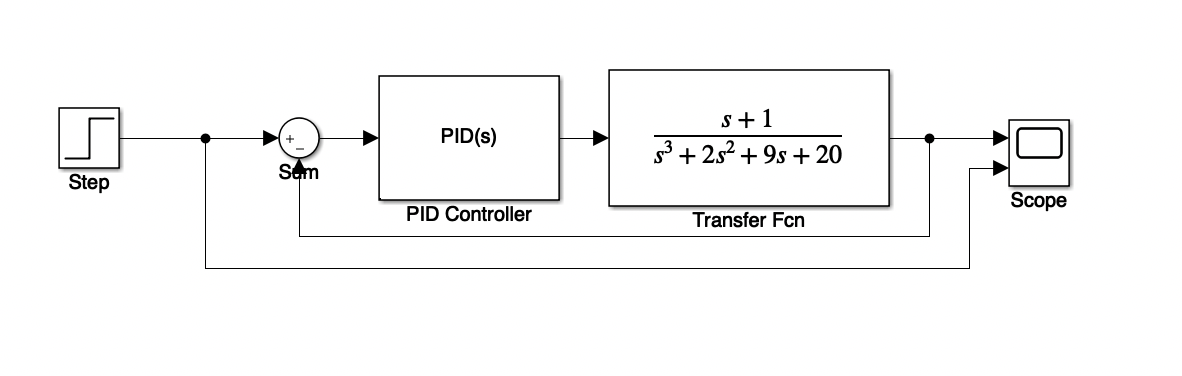
\includegraphics[width=15.5cm, height=7cm]{simulink_pid.png}
$$$$
2. Open pidTuner in Matlab and show parametrs for tuning
$$$$
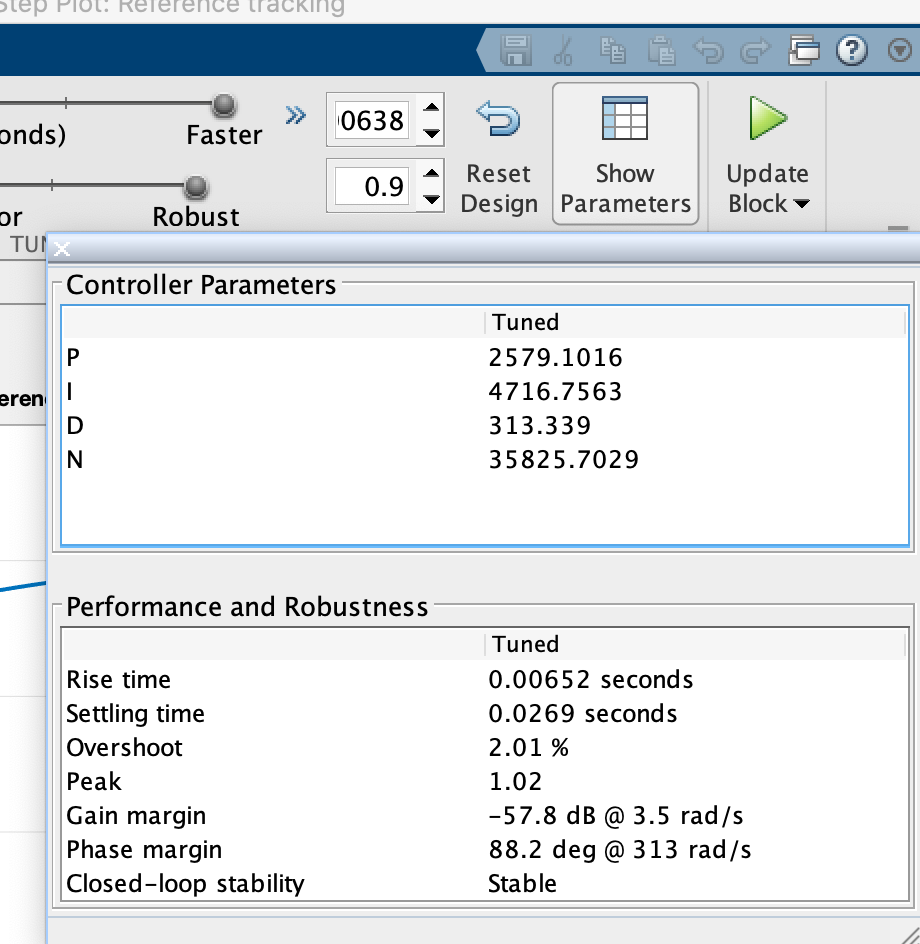
\includegraphics[width=15.5cm, height=10cm]{show_parametrs.png}
$$$$
3. Tune Response time and Transient Behavior
$$$$
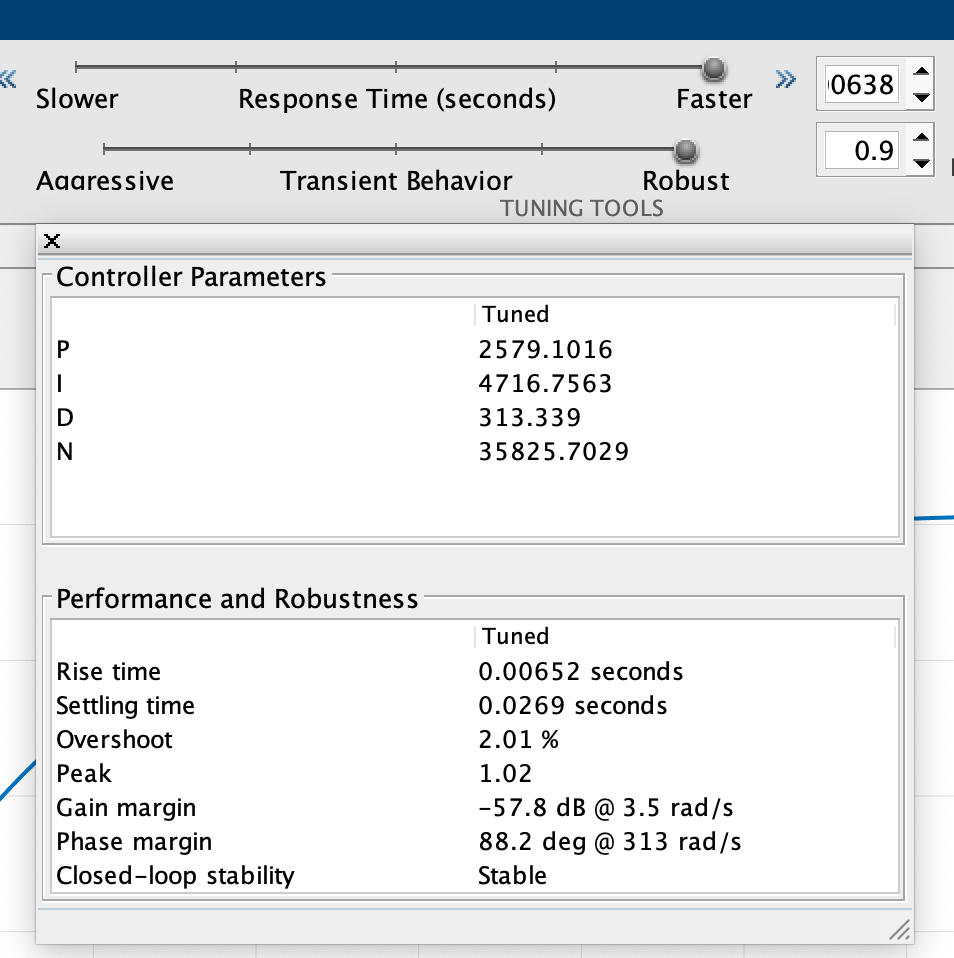
\includegraphics[width=15.5cm, height=10cm]{after_tuning_pid.png}
$$$$
4. Compare results before tuning and after
$$$$
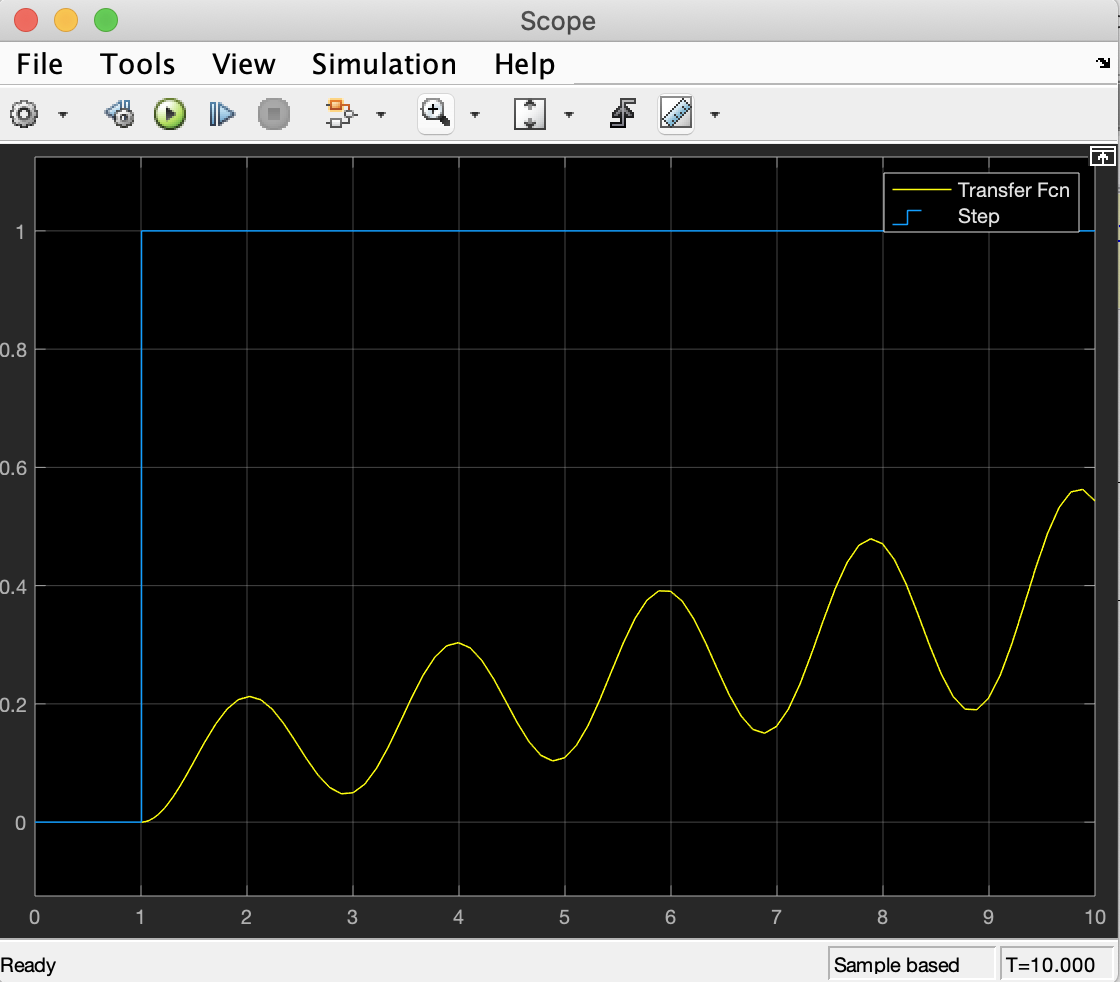
\includegraphics[width=15.5cm, height=10cm]{initial_without_pid.png}
$$$$
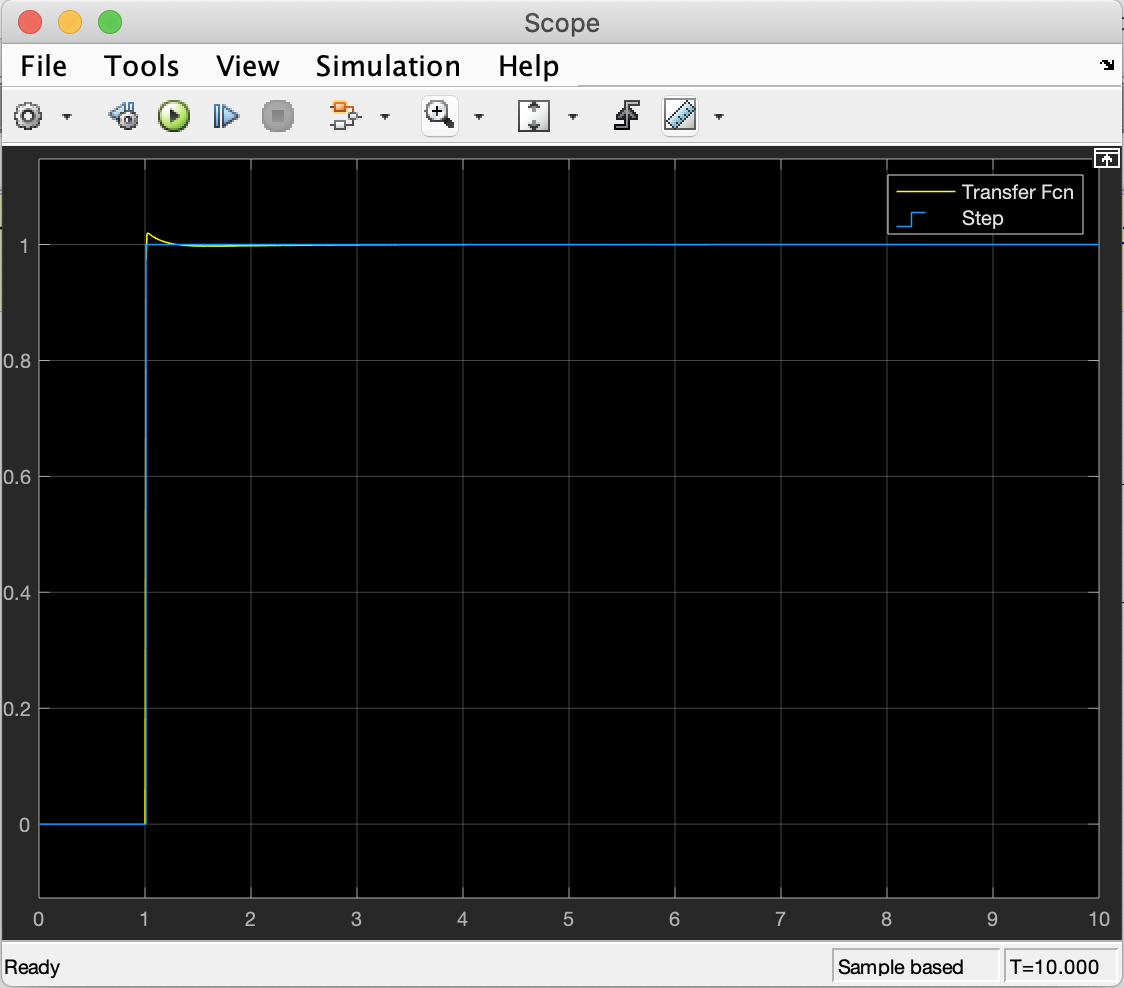
\includegraphics[width=15.5cm, height=10cm]{final_results_pid.png}
$$$$
5. PID parameters
$$$$
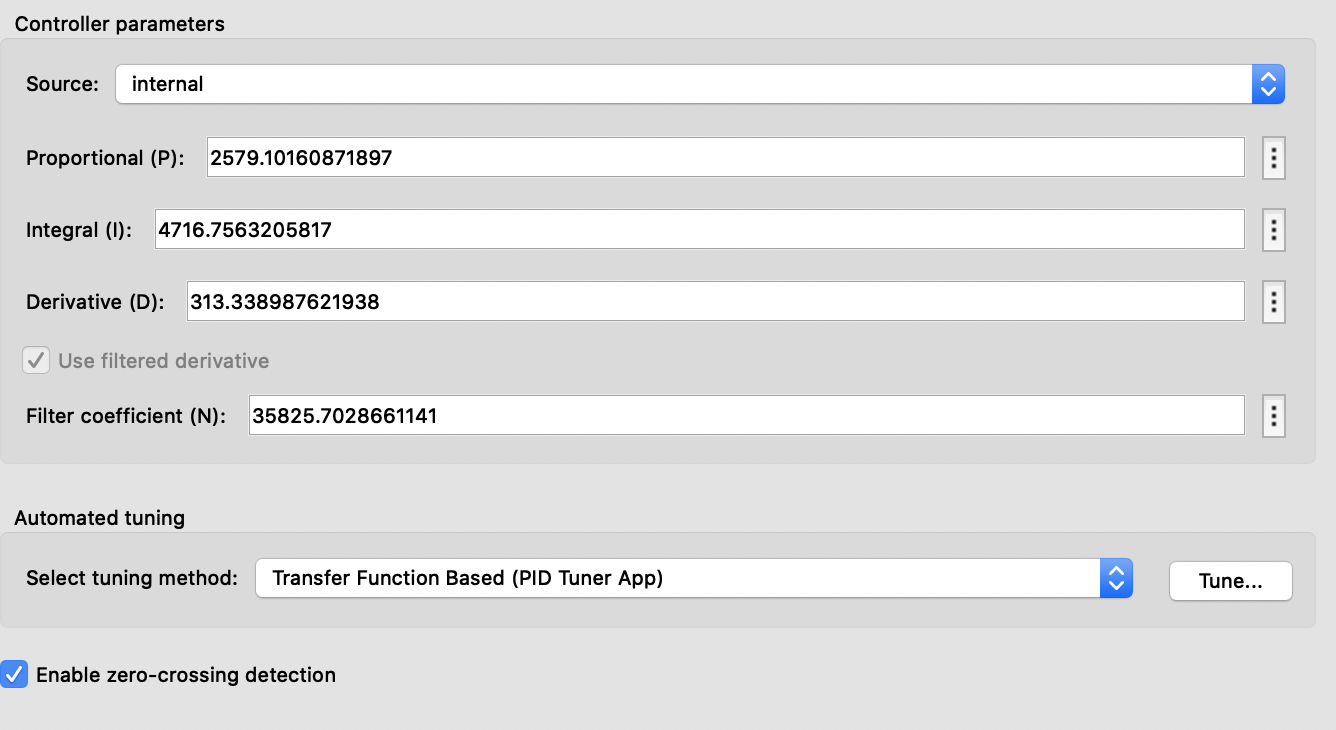
\includegraphics[width=15.5cm, height=10cm]{PID_params.png}
$$$$



\section*{Problem 3}
$$W(s) = \frac{s+2}{s^2 + 4s + 11}$$
\begin{problem}
  \problemquestion{Design a lag or lead compensator (if applicable), play with zero and pole to find optimal values (of overshoot, peak time, transient process time, stationary error, etc.) for transient process. Use editors in Matlab Control System Designer.}
\end{problem}

1. Open Control System Designer in MATLAB
\begin{lstlisting}
>> controlSystemDesigner(tf([1, 2],[1,4,11]))
\end{lstlisting}
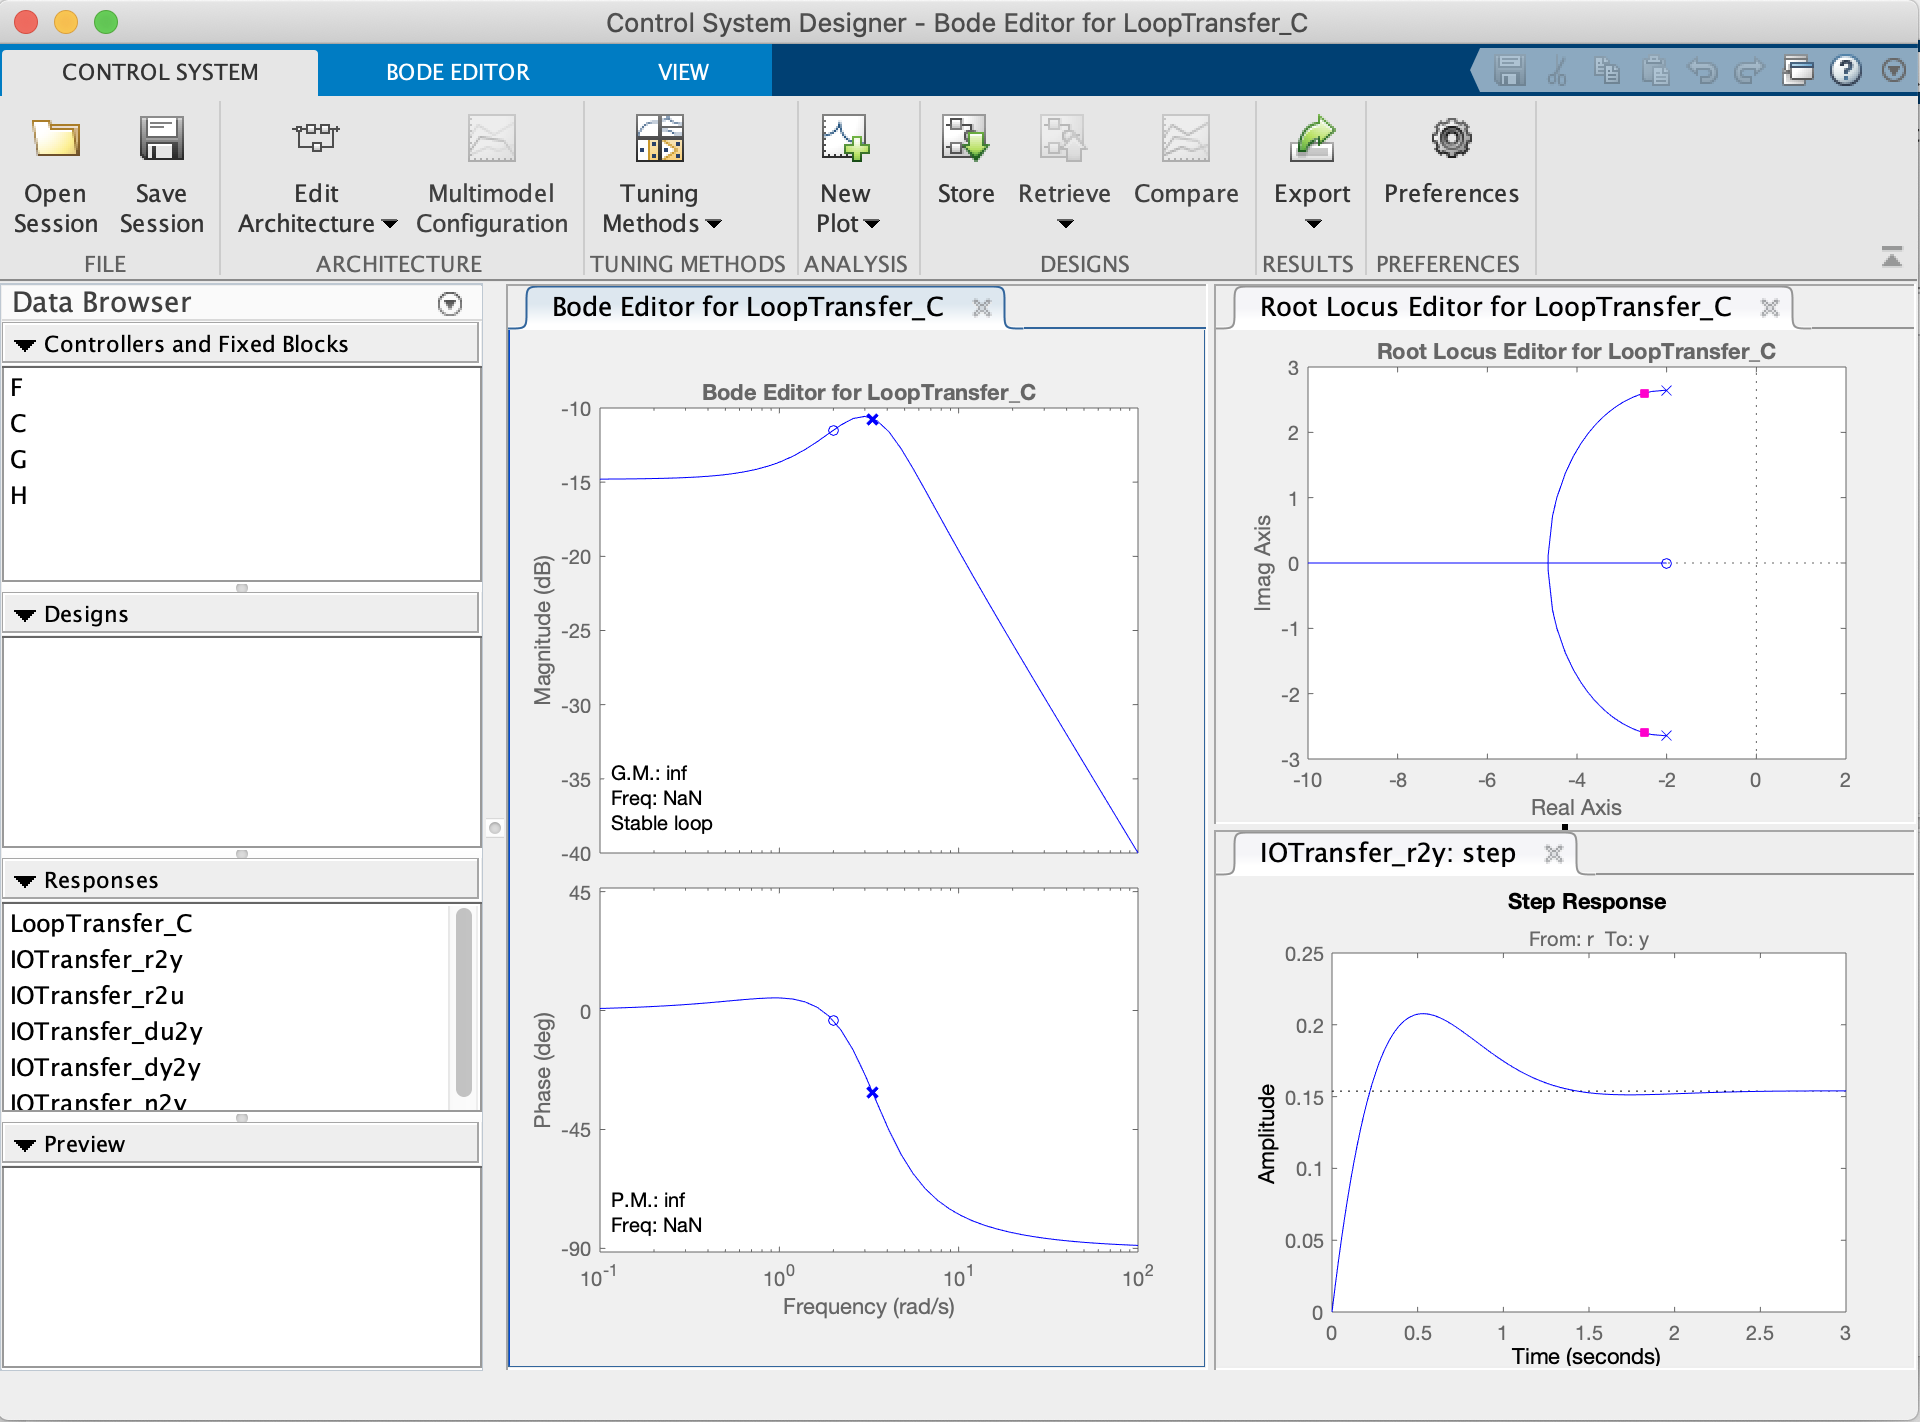
\includegraphics[width=15.5cm, height=10cm]{initial.png}

2. To tune poles and zeros we will use Root Locus plot
$$$$
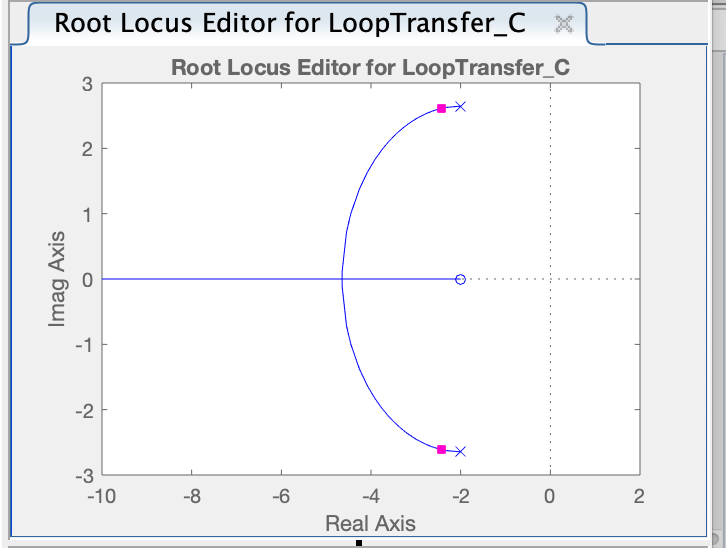
\includegraphics[width=10.5cm, height=5cm]{to_tune.png}
$$$$
3. After tuning we will have following step response
$$$$
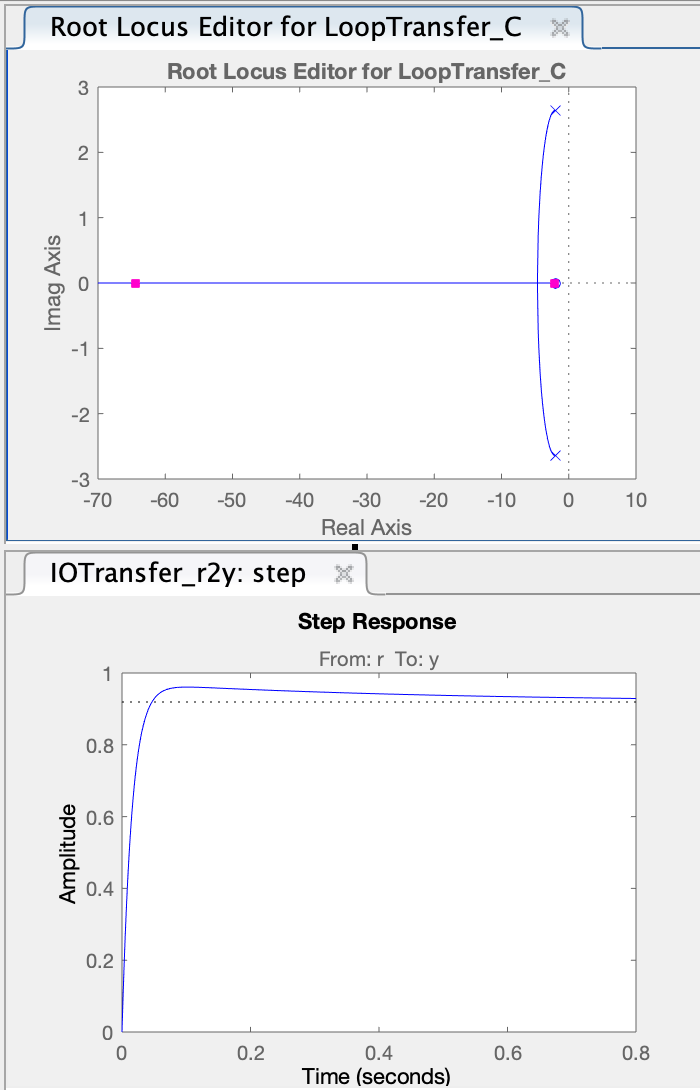
\includegraphics[width=10.5cm, height=10cm]{after_hand_tuned.png}
$$$$
Save results for comparison
$$$$
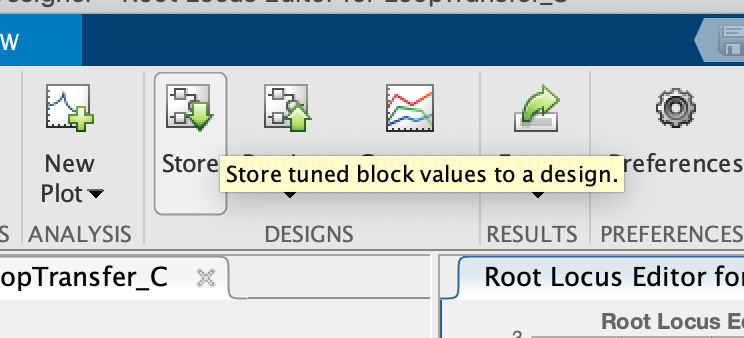
\includegraphics[width=15.5cm, height=10cm]{compare.png}
$$$$
4. To compare results to optimal we will auto-tune with PID tuner
$$$$
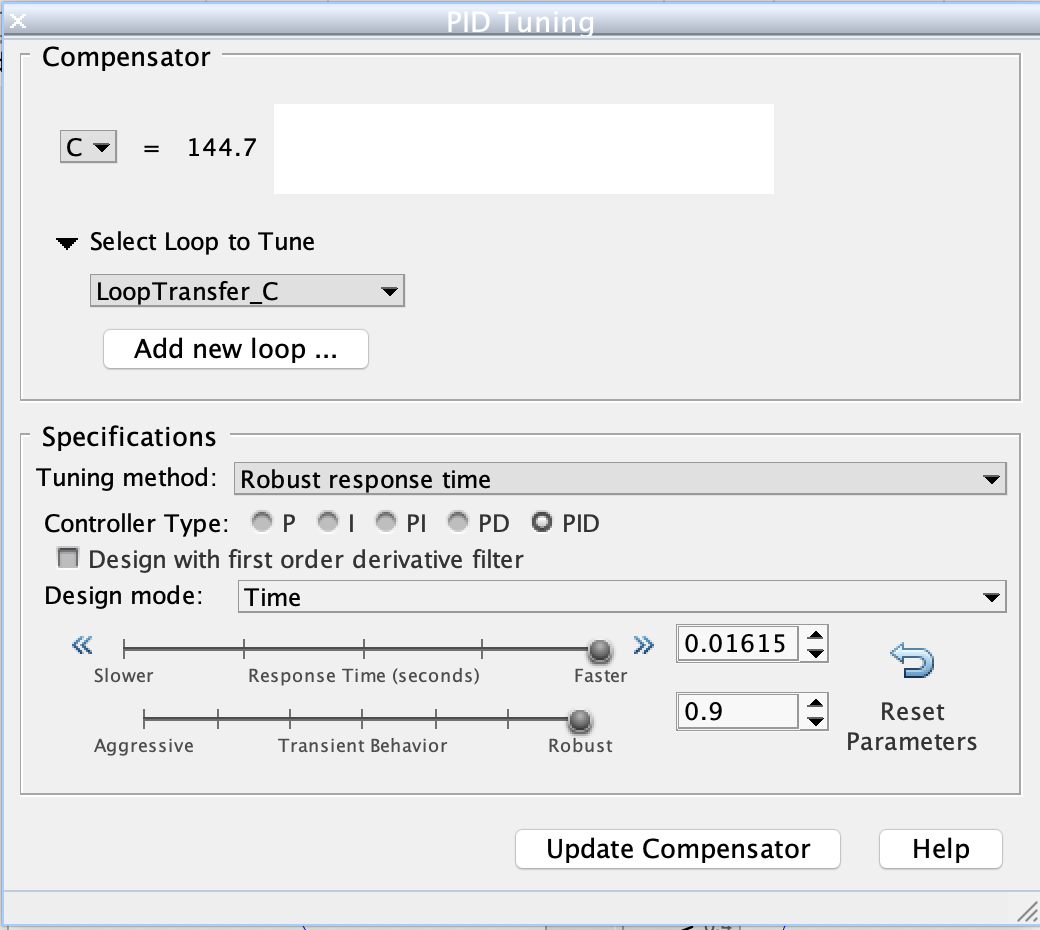
\includegraphics[width=15.5cm, height=10cm]{PID_tuned.png}
$$$$
5. Compare PID tuned results with hand tuned and inital system
$$$$
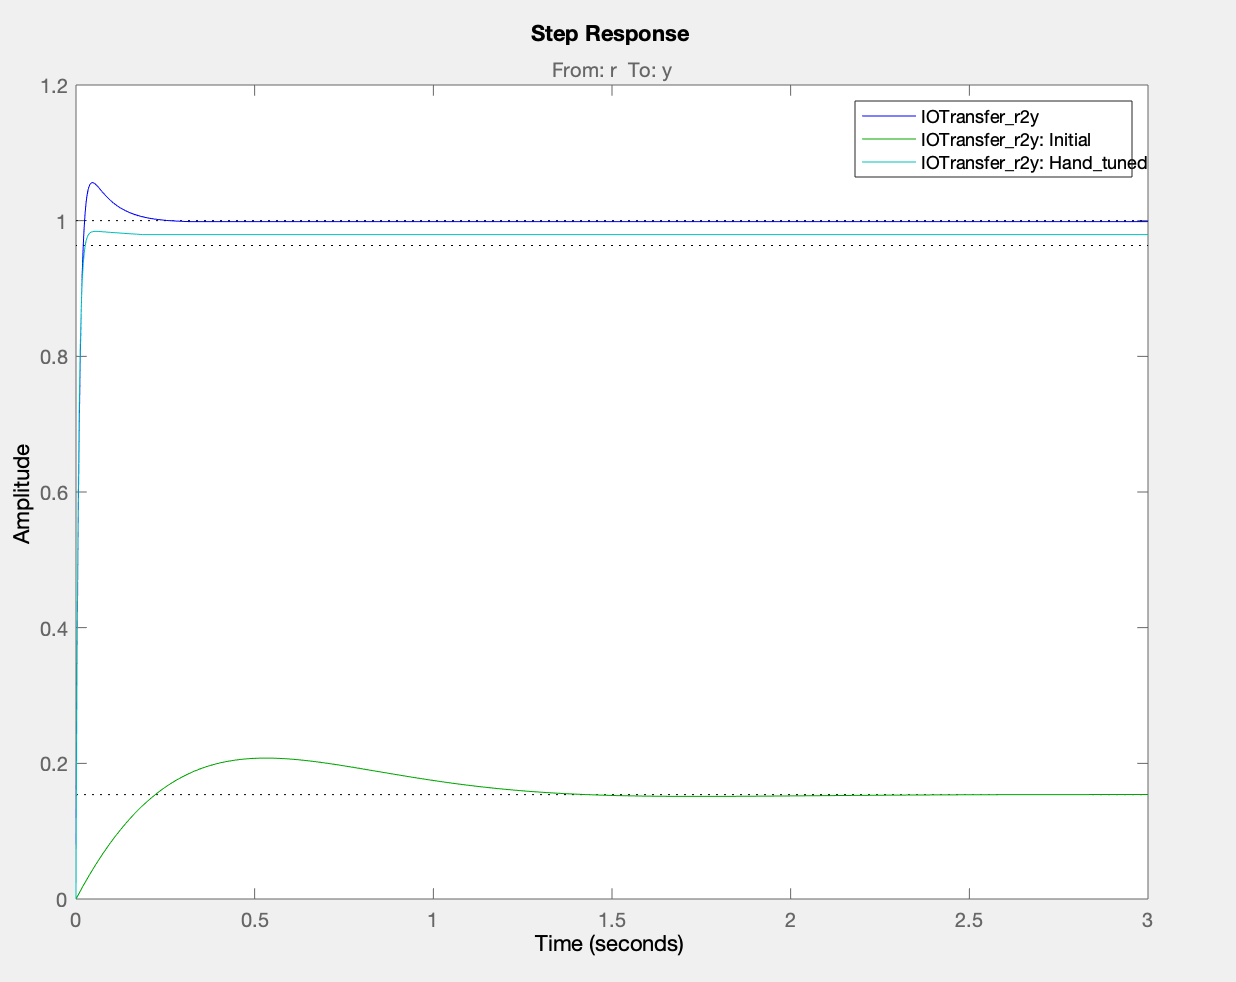
\includegraphics[width=15.5cm, height=10cm]{final_results.png}
$$$$
6. Get designed Lead–lag compensator from following architecute
$$$$
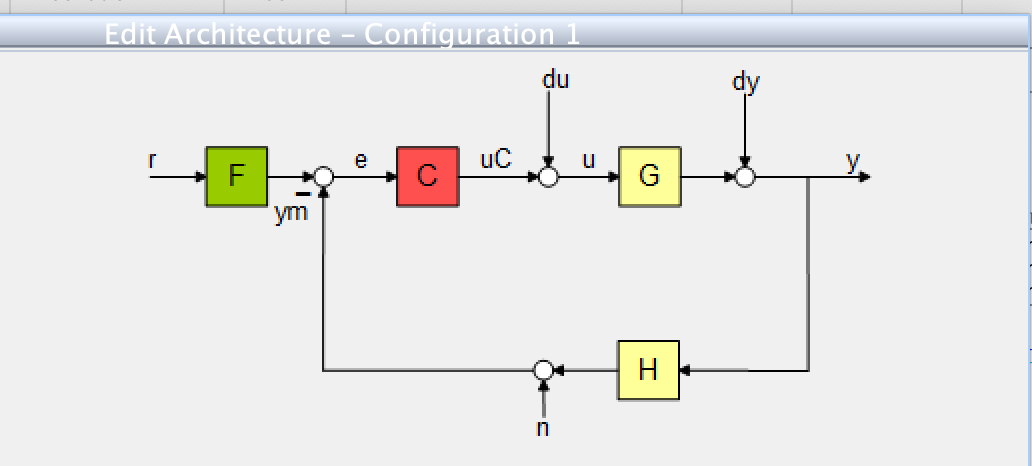
\includegraphics[width=15.5cm, height=10cm]{lag_architecture.png}
$$Answer:C = \frac{0.086947(s+1411)(s+12.89)}{s}$$

\end{document}
